% docs/slides/preamble.tex -- 五份 deck 共享
\documentclass[aspectratio=169,11pt]{beamer}

% ==== 中文与字体 ====
\usepackage[UTF8,fontset=none]{ctex}
\usepackage{fontspec}

\IfFontExistsTF{PingFang SC}{%
  \setCJKmainfont{PingFang SC}[BoldFont=PingFang SC,ItalicFont=PingFang SC,AutoFakeSlant=0.15]
  \setCJKsansfont{PingFang SC}[ItalicFont=PingFang SC,AutoFakeSlant=0.15]
  \setCJKmonofont{PingFang SC}
}{%
  \IfFontExistsTF{Source Han Sans SC}{%
    \setCJKmainfont{Source Han Sans SC}
    \setCJKsansfont{Source Han Sans SC}
  }{%
    \IfFontExistsTF{Noto Sans CJK SC}{%
      \setCJKmainfont{Noto Sans CJK SC}
      \setCJKsansfont{Noto Sans CJK SC}
    }{%
      \setCJKmainfont{Heiti SC}
      \setCJKsansfont{Heiti SC}
    }
  }
}

\IfFontExistsTF{Helvetica Neue}{\setmainfont{Helvetica Neue}}{%
  \IfFontExistsTF{Inter}{\setmainfont{Inter}}{}}
\IfFontExistsTF{JetBrains Mono}{\setmonofont{JetBrains Mono}[Scale=0.85]}%
  {\setmonofont{Menlo}[Scale=0.85]}

% ==== 颜色 ====
\usepackage{xcolor}
\definecolor{cMain}{HTML}{1F4E79}
\definecolor{cAccent}{HTML}{E07A1F}
\definecolor{cGray}{HTML}{595959}
\definecolor{cMute}{HTML}{F4F4F4}
\definecolor{cOK}{HTML}{2E7D32}
\definecolor{cBad}{HTML}{B23A3A}
\definecolor{cWarn}{HTML}{C8A300}

% ==== 主题 ====
\usepackage{tcolorbox}
\usetheme{metropolis}
\metroset{progressbar=frametitle,numbering=fraction,block=fill}
\setbeamercolor{frametitle}{bg=cMain,fg=white}
\setbeamercolor{progress bar}{fg=cAccent,bg=cMute}
\setbeamercolor{alerted text}{fg=cAccent}
\setbeamercolor{title}{fg=cMain}

% metropolis 默认尝试 Fira Sans，未安装时 fallback 到 Latin Modern Sans。
% 这里在主题加载后显式覆盖，强制使用 macOS 上一定存在的 Helvetica Neue，
% 跟中文 PingFang 风格一致；找不到则按顺序尝试 Inter / Arial。
\IfFontExistsTF{Helvetica Neue}{%
  \setsansfont{Helvetica Neue}%
}{%
  \IfFontExistsTF{Inter}{\setsansfont{Inter}}{%
    \IfFontExistsTF{Arial}{\setsansfont{Arial}}{}}%
}

% ==== TikZ ====
\usepackage{tikz}
\usetikzlibrary{positioning,arrows.meta,fit,shapes.geometric,calc,%
  decorations.pathmorphing,backgrounds}

\tikzset{
  node-box/.style={draw=cMain,thick,rounded corners=2pt,
    minimum height=8mm,minimum width=18mm,align=center,font=\small},
  node-state/.style={draw=cMain,thick,circle,minimum size=14mm,
    align=center,font=\small},
  node-ok/.style={draw=cOK,thick,fill=cOK!10},
  node-warn/.style={draw=cWarn,thick,fill=cWarn!15},
  node-bad/.style={draw=cBad,thick,fill=cBad!10},
  % 色盲友好的状态机三态：蓝 (正常/Closed) / 橙 (告警/Open) / 灰 (中间/HalfOpen)
  % 避免 red-green 二元区分，改用 hue + lightness 双通道。
  node-state-normal/.style={draw=cMain,thick,fill=cMain!12},
  node-state-alert/.style={draw=cAccent,thick,fill=cAccent!18},
  node-state-transition/.style={draw=cGray,thick,fill=cGray!18},
  arrow/.style={-{Stealth[length=2mm]},thick,draw=cMain},
  arrow-async/.style={-{Stealth[length=2mm]},thick,dashed,draw=cGray},
  arrow-bad/.style={-{Stealth[length=2mm]},thick,draw=cBad},
  arrow-alert/.style={-{Stealth[length=2mm]},thick,draw=cAccent},
  lifeline/.style={dashed,thick,draw=cGray},
}

% ==== 代码 ====
\usepackage{listings}
\lstdefinelanguage{Go}{
  morekeywords={break,case,chan,const,continue,default,defer,else,
    fallthrough,for,func,go,goto,if,import,interface,map,package,range,
    return,select,struct,switch,type,var,nil,true,false,iota},
  morekeywords=[2]{string,int,int64,uint,uint64,bool,byte,error,context},
  sensitive=true,
  morecomment=[l]//,morecomment=[s]{/*}{*/},
  morestring=[b]",morestring=[b]`,
}
\lstdefinelanguage{LuaRedis}{
  morekeywords={and,break,do,else,elseif,end,false,for,function,if,in,
    local,nil,not,or,repeat,return,then,true,until,while},
  morekeywords=[2]{redis,call,KEYS,ARGV,tonumber,HGET,HSET,GET,SET,
    DECR,DECRBY,INCR,INCRBY,EXPIRE,PEXPIRE,ZADD,ZCARD,ZREMRANGEBYSCORE,
    EVAL,EVALSHA},
  sensitive=true,
  morecomment=[l]{--},
  morestring=[b]",morestring=[b]',
}

\lstdefinestyle{base}{
  basicstyle=\ttfamily\scriptsize,
  numbers=left,numberstyle=\tiny\color{cGray},
  keywordstyle=\color{cMain}\bfseries,
  keywordstyle=[2]\color{cAccent},
  stringstyle=\color{cOK},
  commentstyle=\color{cGray}\itshape,
  backgroundcolor=\color{cMute},
  frame=single,framerule=0pt,
  showstringspaces=false,
  breaklines=true,
  tabsize=2,
  columns=fullflexible,
}
\lstset{style=base}

% ==== 三线表与附录页码 ====
\usepackage{booktabs}
\usepackage{appendixnumberbeamer}

% ==== 页脚来源标注 ====
\newcommand{\srcnote}[1]{{\color{cGray}\scriptsize\itshape #1}}

% 关键论点框
\newcommand{\keypoint}[1]{%
  \begin{tcolorbox}[colback=cMute,colframe=cMain,boxrule=0.5pt,arc=2pt]%
  #1\end{tcolorbox}}


\title{幂等中间件设计}
\subtitle{从 Idempotency-Key 到 Redis Lua 状态机}
\author{gomall · 后端实战}
\date{}

\begin{document}

% ============== 1. 封面 ==============
\maketitle

% ============== 2. 目录 ==============
\begin{frame}{今日大纲}
\tableofcontents
\end{frame}

% ============== 3. 故事开场 ==============
\section{为什么需要幂等}

\begin{frame}{凌晨两点的电话}
\begin{itemize}
  \item 用户在 App 点了一次"确认支付"。
  \item 网络抖动，前端转圈不动，他烦了，连点了三下。
  \item 第二天客服群炸了：同一笔订单扣了三次款。
\end{itemize}
\vspace{2mm}
\keypoint{重复请求只生效一次 —— 这就是幂等。}
\srcnote{源自 docs/blog/01-idempotency.md \S 一个让人崩溃的场景}
\end{frame}

\begin{frame}{重复请求的四种来源}
\begin{tikzpicture}[node distance=8mm and 8mm,
    every node/.append style={minimum width=15mm}]
  \node[node-box] (cli) {Client};
  \node[node-box,right=of cli] (cdn) {CDN/LB};
  \node[node-box,right=of cdn] (gw)  {API GW};
  \node[node-box,right=of gw]  (bff) {BFF};
  \node[node-box,right=of bff] (svc) {Service};
  \draw[arrow] (cli) -- (cdn);
  \draw[arrow] (cdn) -- (gw);
  \draw[arrow] (gw)  -- (bff);
  \draw[arrow] (bff) -- (svc);
  \draw[arrow-bad,bend right=35] (cli) to node[below,font=\tiny]{用户狂点} (cdn);
  \draw[arrow-bad,bend right=35] (cdn) to node[below,font=\tiny]{网关重投} (gw);
  \draw[arrow-bad,bend right=35] (gw)  to node[below,font=\tiny]{超时重试} (bff);
  \draw[arrow-bad,bend right=35] (bff) to node[below,font=\tiny]{MQ 重投} (svc);
\end{tikzpicture}
\vspace{2mm}
\small 任何一层都能制造重复 —— 服务端必须假设"上游每个请求都可能重发"。
\end{frame}

% ============== 4. 错法 ==============
\section{两个常见错法}

\begin{frame}[fragile]{错法一：唯一索引硬扛}
\begin{lstlisting}[language=SQL,basicstyle=\ttfamily\scriptsize]
CREATE UNIQUE INDEX uk_user_token
  ON orders (user_id, idempotency_token);
\end{lstlisting}
\begin{itemize}
  \item 第一次插入成功，第二次冲突 \texttt{1062 Duplicate}。
  \item 但客户端拿不到第一次的响应体 —— 它需要订单号。
  \item 跨表场景失效：扣库存、写积分、发券都需要独立 token。
\end{itemize}
\srcnote{对应 docs/blog/01-idempotency.md \S 错误的做法 1}
\end{frame}

\begin{frame}{错法二：先 GET 再 SET 的竞态}
\begin{tikzpicture}[node distance=10mm]
  \foreach \name/\x in {A 线程/0, B 线程/30, Redis/60} {
    \node[node-box,minimum width=14mm] at (\x mm,0) (\name) {\name};
    \draw[lifeline] (\x mm,-2mm) -- (\x mm,-42mm);
  }
  \draw[arrow] (0,-8mm)  -- node[above,font=\tiny]{GET token} (60mm,-8mm);
  \draw[arrow] (30mm,-14mm) -- node[above,font=\tiny]{GET token} (60mm,-14mm);
  \draw[arrow-bad] (60mm,-20mm) -- node[above,font=\tiny\color{cBad}]{两条都返回 nil} (0,-20mm);
  \draw[arrow-bad] (60mm,-26mm) -- node[above,font=\tiny\color{cBad}]{两条都返回 nil} (30mm,-26mm);
  \draw[arrow] (0,-32mm)  -- node[above,font=\tiny]{SET processing} (60mm,-32mm);
  \draw[arrow] (30mm,-38mm) -- node[above,font=\tiny]{SET processing} (60mm,-38mm);
\end{tikzpicture}
\vspace{1mm}
\small 两个线程都判断"没占用"$\to$ 两次都进入业务 $\to$ 还是重复扣款。
\end{frame}

% ============== 5. 正解 ==============
\section{三态机正解}

\begin{frame}{正解：状态机 + Lua + 响应回放}
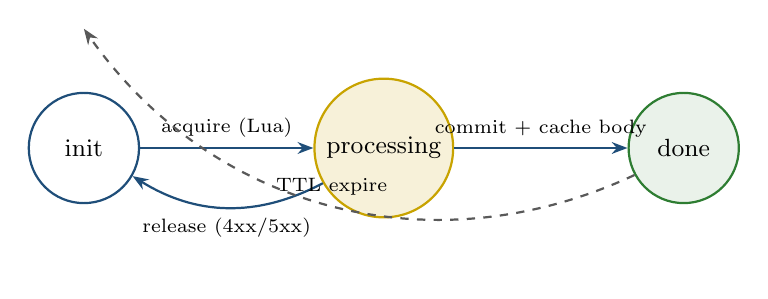
\begin{tikzpicture}[node distance=22mm]
  \node[node-state] (init) {init};
  \node[node-state,node-warn,right=of init] (proc) {processing};
  \node[node-state,node-ok,right=of proc] (done) {done};

  \draw[arrow] (init) -- node[above,font=\scriptsize]{acquire (Lua)} (proc);
  \draw[arrow] (proc) -- node[above,font=\scriptsize]{commit + cache body} (done);
  \draw[arrow,bend left=30] (proc) to node[below,font=\scriptsize]{release (4xx/5xx)} (init);
  \draw[arrow-async,bend left=40] (done) to node[above,font=\scriptsize]{TTL expire} ([yshift=8mm]init.north);
\end{tikzpicture}
\vspace{2mm}
\small \textbf{三种命中}：1 拿锁 / 2 回放 done / 3 处理中拒绝 / 0 token 不存在。
\end{frame}

\begin{frame}{acquire 四种返回的语义}
\begin{tabular}{@{}lll@{}}
\toprule
返回码 & 含义 & 服务端响应 \\
\midrule
1 & init$\to$processing 成功 & 进入业务逻辑 \\
2 & 命中 done，附 result & 回放缓存的响应体 \\
3 & 命中 processing & 返回"处理中"，让客户端等待 \\
0 & token 不存在 & 返回"token 无效或过期" \\
\bottomrule
\end{tabular}
\vspace{3mm}
\keypoint{四种返回必须在一段 Lua 里判定，否则就是"先 GET 再 SET"的换皮。}
\srcnote{repository/cache/idempotency.go:32--50}
\end{frame}

\begin{frame}[fragile]{Lua 脚本完整实现}
\begin{lstlisting}[language=LuaRedis,firstnumber=32,
  caption={\srcnote{repository/cache/idempotency.go:32--50}}]
local v = redis.call('HGET', KEYS[1], 'state')
if v == false or v == nil then
    return {0, ''}
end
if v == 'done' then
    local r = redis.call('HGET', KEYS[1], 'result')
    return {2, r or ''}
end
if v == 'processing' then
    return {3, ''}
end
if v == 'init' then
    redis.call('HSET', KEYS[1], 'state', 'processing')
    redis.call('EXPIRE', KEYS[1], tonumber(ARGV[1]))
    return {1, ''}
end
return {0, ''}
\end{lstlisting}
\end{frame}

\begin{frame}{为什么必须 Lua}
\begin{itemize}
  \item Redis 单线程串行执行命令，但 GET + SET 是\textbf{两条独立命令}，中间会被其他客户端插入。
  \item Lua 脚本对外是一条"原子命令"：所有 KEYS 操作在脚本运行期间不会被打断。
  \item 写 Lua 还有一个好处：把"返回码语义"封进脚本，调用方只关心 1/2/3/0。
\end{itemize}
\vspace{2mm}
\keypoint{Lua $\ne$ 分布式锁，它是把"check-then-act"装进一条原子命令的工具。}
\end{frame}

% ============== 6. 中间件实现 ==============
\section{中间件落地}

\begin{frame}[fragile]{用户隔离的 key 命名}
\begin{lstlisting}[language=Go,firstnumber=15,
  caption={\srcnote{repository/cache/key.go:15--21}}]
const IdempotencyKey = "idemp:%d:%s"

func IdempotencyTokenKey(userId uint, token string) string {
    return fmt.Sprintf(IdempotencyKey, userId, token)
}
\end{lstlisting}
\vspace{1mm}
\small 不用 \texttt{idemp:\{token\}}：避免恶意用户预测 token 抢占别人的请求，也方便按用户清理。
\end{frame}

\begin{frame}[fragile]{responseRecorder：拿到 gin 的响应体}
\begin{lstlisting}[language=Go,firstnumber=18,
  caption={\srcnote{middleware/idempotency.go:18--31}}]
type responseRecorder struct {
    gin.ResponseWriter
    body *bytes.Buffer
}

func (r *responseRecorder) Write(b []byte) (int, error) {
    r.body.Write(b)
    return r.ResponseWriter.Write(b)
}

func (r *responseRecorder) WriteString(s string) (int, error) {
    r.body.WriteString(s)
    return r.ResponseWriter.WriteString(s)
}
\end{lstlisting}
\end{frame}

\begin{frame}[fragile]{中间件主干}
\begin{lstlisting}[language=Go,firstnumber=60,
  caption={\srcnote{middleware/idempotency.go:60--111}}]
key := cache.IdempotencyTokenKey(user.Id, token)
state, cached, err := cache.AcquireIdempotencyLock(c.Request.Context(), key)
switch state {
case 2: // done -> 回放
    c.Header("X-Idempotent-Replay", "true")
    c.Data(http.StatusOK, "application/json", []byte(cached))
    c.Abort(); return
case 3: c.JSON(200, gin.H{"msg":"处理中"}); c.Abort(); return
case 0: c.JSON(200, gin.H{"msg":"token 无效"}); c.Abort(); return
}
recorder := &responseRecorder{ResponseWriter: c.Writer, body: bytes.NewBuffer(nil)}
c.Writer = recorder
c.Next()
if len(c.Errors) > 0 || recorder.Status() >= 400 {
    cache.ReleaseIdempotencyLock(c.Request.Context(), key); return
}
cache.CommitIdempotencyResult(c.Request.Context(), key, recorder.body.String())
\end{lstlisting}
\end{frame}

\begin{frame}{第二次请求的完整时序}
\begin{tikzpicture}[node distance=10mm]
  \foreach \name/\x in {Client/0, Mw/30, Redis/60, Biz/90} {
    \node[node-box,minimum width=14mm] at (\x mm,0) (\name) {\name};
    \draw[lifeline] (\x mm,-2mm) -- (\x mm,-55mm);
  }
  \draw[arrow] (0,-8mm) -- node[above,font=\tiny]{POST + Idempotency-Key} (30mm,-8mm);
  \draw[arrow] (30mm,-14mm) -- node[above,font=\tiny]{EVAL acquire} (60mm,-14mm);
  \draw[arrow] (60mm,-20mm) -- node[above,font=\tiny]{return \{2, result\}} (30mm,-20mm);
  \draw[arrow-async] (30mm,-30mm) -- node[below,font=\tiny,text=cGray]{Biz 完全不被触发} (90mm,-30mm);
  \draw[arrow] (30mm,-42mm) -- node[above,font=\tiny]{200 + X-Idempotent-Replay: true} (0,-42mm);
  \node[font=\scriptsize,text=cGray] at (45mm,-50mm)
    {p95 2.33ms，比第一次下单快一个数量级};
\end{tikzpicture}
\end{frame}

\begin{frame}{失败回滚 vs 永久死锁}
\begin{itemize}
  \item 业务返回 4xx/5xx 时 \texttt{ReleaseIdempotencyLock} 将状态打回 \texttt{init}。
  \item 客户端拿同一 token 重试时，可以重新进入 \texttt{processing}。
  \item 若失败也写 \texttt{done}：客户端重试只能拿到上次的错误响应，永远卡死。
\end{itemize}
\vspace{2mm}
\keypoint{processing $\to$ init 是状态机里最容易被忽视的一条边。}
\srcnote{middleware/idempotency.go:101--105 + repository/cache/idempotency.go:87--90}
\end{frame}

% ============== 7. 性能 ==============
\section{压测数据}

\begin{frame}{50 VU $\times$ 15s = 755{,}033 请求}
\begin{tabular}{@{}lr@{}}
\toprule
指标 & 数值 \\
\midrule
压测脚本 & \texttt{idempotency\_replay.js} \\
VU 数 & 50 \\
时长 & 15s \\
总请求 & \textbf{755{,}033} \\
DB 实际订单 & \textbf{1} \\
\bottomrule
\end{tabular}
\vspace{3mm}
\keypoint{750K 个 POST，DB 落 1 笔 —— 这是中间件应有的"过滤强度"。}
\srcnote{stressTest/REPORT.md \S 4. 幂等中间件}
\end{frame}

\begin{frame}{延迟分布：回放比真实下单快 5 倍}
\begin{tabular}{@{}lrrrr@{}}
\toprule
链路 & RPS & p50 & p95 & max \\
\midrule
Ping 基线 & 64{,}254 & 0.91ms & 3.51ms & 109ms \\
幂等下单 (回放) & \textbf{50{,}319} & 0.50ms & \textbf{2.33ms} & 73ms \\
\bottomrule
\end{tabular}
\vspace{3mm}
\small 回放路径只走 Redis Hash + Lua，避免了下单完整链路里的事务、库存预扣、Outbox 写入。
\srcnote{stressTest/REPORT.md \S 链路压测表 第 1 行 + 第 4 行}
\end{frame}

% ============== 8. 设计取舍 ==============
\section{设计取舍}

\begin{frame}{TTL 选 5 分钟，怎么定？}
\begin{itemize}
  \item 太短：客户端重试网络往返 1--2s，token 提前过期会让重试变成新请求。
  \item 太长：占用 Redis 内存；如果 token 泄漏，攻击者能长期复用。
  \item 5 分钟：覆盖单次业务的所有重试窗口，过期后客户端必须重新申请。
\end{itemize}
\srcnote{repository/cache/idempotency.go:16--17 \texttt{IdempotencyTokenTTL = 5 * time.Minute}}
\end{frame}

\begin{frame}{Redis 挂了，怎么 fail？}
\begin{itemize}
  \item 选 fail-close：Lua 报错时返回 5xx，\textbf{不放行}业务。
  \item 选 fail-open：Lua 报错继续走业务 —— 等于关闭幂等保护。
  \item 钱相关接口必须 fail-close，宁可短时全断也不能漏一笔重复扣款。
\end{itemize}
\vspace{2mm}
\keypoint{安全默认 (safe default) = 失败方向选"对用户负责"的那一边。}
\srcnote{middleware/idempotency.go:61--69}
\end{frame}

\begin{frame}{幂等 vs 分布式锁 vs 去重表}
\begin{tabular}{@{}lll@{}}
\toprule
机制 & 解决的问题 & 典型用法 \\
\midrule
幂等中间件 & 重复\textbf{请求}只生效一次 & 下单/支付/退款 \\
分布式锁 & 同一资源同时\textbf{只有一个执行者} & 定时任务、库存合并扣减 \\
去重表 & 已处理的\textbf{业务 id} 不再处理 & MQ 消费端、回调接收 \\
\bottomrule
\end{tabular}
\vspace{3mm}
\small 三者都关心"避免重复"，但作用维度不同 —— 面试时一定要区分清楚。
\end{frame}

% ============== 9. Q&A ==============
\appendix

\begin{frame}{面试 Q\&A（上）}
\textbf{Q1}：为什么"先 GET 再 SET"不是幂等？\\
\hspace{4mm}\small A：两条命令之间存在竞态，必须用 Lua 原子化。

\vspace{2mm}
\textbf{Q2}：客户端没拿到响应就重试，怎么避免重复扣款？\\
\hspace{4mm}\small A：第二次进入命中 done，回放上一次缓存的响应体，业务不再执行。

\vspace{2mm}
\textbf{Q3}：幂等 token 的生命周期谁来负责？TTL 设多长？\\
\hspace{4mm}\small A：服务端发 token + 设 TTL；5 分钟覆盖单次业务的重试窗口。
\end{frame}

\begin{frame}{面试 Q\&A（下）}
\textbf{Q4}：业务处理失败，token 状态怎么回滚？\\
\hspace{4mm}\small A：processing $\to$ init，让同 token 还能重试；不能写 done 否则永久卡死。

\vspace{2mm}
\textbf{Q5}：幂等 vs 分布式锁的边界？\\
\hspace{4mm}\small A：幂等让同一请求只生效一次；锁让同一资源同时只有一个执行者。

\vspace{2mm}
\textbf{反追问}：跨方法能共用 token 吗？\texttt{Idempotency-Key} 是不是规范？\\
\hspace{4mm}\small A：不建议跨方法共用；这个 Header 名是 IETF 草案 \texttt{draft-ietf-httpapi-idempotency-key-header}。
\end{frame}

\begin{frame}{代码位置一览}
\begin{description}
  \item[中间件主干]\srcnote{middleware/idempotency.go:35--112}
  \item[Lua 脚本]\srcnote{repository/cache/idempotency.go:32--50}
  \item[acquire 包装]\srcnote{repository/cache/idempotency.go:64--76}
  \item[commit / release]\srcnote{repository/cache/idempotency.go:79--90}
  \item[key 命名]\srcnote{repository/cache/key.go:19--21}
  \item[压测脚本]\srcnote{stressTest/idempotency\_replay.js}
\end{description}
\vspace{3mm}
\keypoint{复现：\texttt{k6 run stressTest/idempotency\_replay.js}}
\end{frame}

\end{document}
